\documentclass[12pt]{article}
\usepackage[spanish,mexico]{babel}
	\selectlanguage{spanish}
\usepackage{graphicx}
\usepackage{amsmath}
\usepackage{wrapfig}
\usepackage[dvipsnames]{xcolor}
\usepackage{float}
\usepackage{multicol}
\usepackage{geometry}
\usepackage{hyperref}
\usepackage[utf8]{inputenc}

\newgeometry{top=2cm}

\title{Actividad 7: El Espacio Fase}
\author{Ana Gabriela Carretas Talamante}
\date{17 de marzo de 2016}

\begin{document}
\maketitle
\section{Introducción}

La ecuación diferencial que representa el movimiento de un péndulo simple es:
\begin{equation}
\label{1}
\frac{d^2\theta}{dt^2} + \frac{g}{l}\sin\theta=0
\end{equation}
donde $g$ es la aceleración causada por la gravedad, $l$ es la longitud del péndulo y $\theta$ es el desplazamiento angular \cite{W}. \\

En actividades pasadas hemos estado trabajando con la ecuación mostrada anteriormente, ya sea resolviéndola o integrando componentes que salen de ella. En esta ocasión, se nos ha encargado mapear el espacio fase de soluciones para la ecuación diferencial, que mostrara las posibles soluciones dependiendo de las condiciones iniciales. \\

\begin{figure}[H]
\centering
   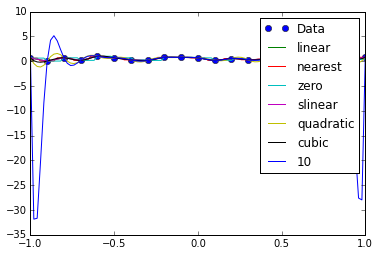
\includegraphics[width=7cm]{1}
  \caption{Espacio fase de un péndulo simple \cite{P}.}
\end{figure}

El \textbf{espacio fase} es una representación geométrica de todas las trayectorias de un sistema dinámico no plano. Cada curva representa una condición inicial diferente. Un retrato de fase es una herramienta valiosa en el estudio de los sistemas dinámicos autónomos de segundo orden. La configuración de las curvas en el espacio de fase revela información sobre la existencia de atractores, repulsores, ciclos límite, entre otras cosas \cite{EF}. Cada línea mostrada en el espacio fase representa un par de condiciones iniciales, al ser una solución cíclica, se forman círculos en lugares donde las condiciones son estables y líneas onduladas no cerradas cuando las condiciones iniciales no propician un lugar de equilibrio para el sistema. \\

El método \textit{scipy.integrate.odeint}, que utilizamos en la actividad 5, nos ayuda a resolver ecuaciones diferenciales ordinarias al transformarlas en ecuaciones de primer orden por medio de un cambio de variable. De esta manera, podemos obtener una solución numérica para la ecuación. 

\subparagraph*{Programa: Espacio fase de un péndulo simple.}

Se presenta a continuación el código realizado, en donde se simularon diferentes casos en donde variaron las condiciones iniciales. El código tiene la opción de ajustar los límites de condiciones iniciales, qué tantas líneas se han de graficar, los mapas de colores utilizados y la densidad de estas gráficas, según se declare en las condiciones iniciales del programa. No se incluyen las flechas de campo, no supe cómo ponerlas. 

{\color{PineGreen}\begin{verbatim}
#Exportando mi programa para resolver la ecuacion diferencial 
#del movimiento del pendulo
#Programa editado para múltiples casos
from scipy.integrate import odeint
import numpy as np
import matplotlib.pyplot as plt

#Definimos las constantes 
g=9.8             #Valor de la gravedad
l=0.5             #Longitud de la cuerda
b=0               #Amortiguamiento
c=g/l             #Frecuencia
theta=np.pi/3     #Angulo inicial
omega=0           #Velocidad inicial

theta0=4*np.pi    #Para el espacio fase (thanks Olga)

#Definimos la función para el caso general; incluyendo el amortiguamiento
def pend(y, t, b, c):
     theta, omega = y
     dydt = [omega, -b*omega - c*np.sin(theta)]
     return dydt

#Definimos CI y el intervalo de tiempo
#Doble grafica para rellenar los ojitos
#con una no se alcanzan a apreciar todas las trayectorias
y00 = np.array([-theta0, theta0])
y11 = np.array([-theta0-np.pi,0])

t = np.linspace(0, 10, 1000)

#Para que se vea bonito
#Escala normal y que tan tupida esta esta cosa
values  = linspace(-1.1,1.1,250)

vcolors0 = plt.cm.BrBG(linspace(-3, 3, len(values)))
vcolors1 = plt.cm.BrBG(linspace(1, -1, len(values)))

#Esto se lo copie al Martin, nsqp
plt.figure(2)
#Solo era eso Martin, jaja salu2
#-------------------------------------------------------
#Dibujando las trayectorias
for v, col in zip(values, vcolors0):
    y0 = v * y00                               
    X = odeint(pend, y0, t, args=(b, c))       
    plt.plot( X[:,0], X[:,1], lw=v, color=col, 
    label='X0=(%.f, %.f)' % ( y0[0], y0[1]) )
    
for v, col in zip(values, vcolors1):
    y0 = v * y11                              
    X = odeint(pend, y0, t, args=(b, c))      
    plt.plot( X[:,0], X[:,1], lw=v, color=col, 
    label='X0=(%.f, %.f)' % ( y0[0], y0[1]) )

#-------------------------------------------------------
#Se supone que deberia poner una malla con flechitas
#I don't get it :s
#Asi que no lo pondre
#-------------------------------------------------------
#Graficando suave
plt.title('Trajectories and direction fields')
plt.xlabel('Angle')
plt.xlim(-theta0+2*np.pi,theta0-2*np.pi)
plt.ylabel('Angular velocity')
plt.grid()

#Pa' guardar la foto sin problemas
fig = matplotlib.pyplot.gcf()
fig.set_size_inches(15.5,10.5)
fig.savefig('phaseportrait.png',dpi=100)
\end{verbatim}}

\begin{figure}[H]
\centering
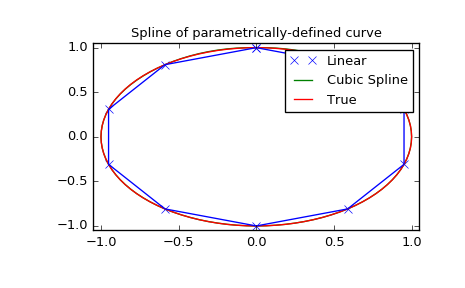
\includegraphics[width=16cm]{2}
\caption{Espacio fase generado para las condiciones iniciales $\theta=\pi/3, \omega=0 \frac{rad}{s}$.}
\end{figure}

\pagebreak

\begin{thebibliography}{6}

\bibitem{W}
Wikipedia,
\emph{Pendulum}. Recuperado en febrero de 2016 de \url{https://en.wikipedia.org/wiki/Pendulum\_(mathematics)}

\bibitem{P}
Krishnavedala,
\emph{Potential energy and phase portrait of a simple pendulum}. Recuperado en marzo de 2016 de \url{https://en.wikipedia.org/wiki/Phase_portrait#/media/File:Pendulum_phase_portrait.svg}

\bibitem{EF}
Wikipedia,
\emph{Retrato de fase}. Recuperado en marzo de 2016 de \url{https://es.wikipedia.org/wiki/Retrato_de_fase}

\bibitem{S1}
Scipy,
\emph{odeint}. \url{http://scipy.github.io/devdocs/generated/scipy.integrate.odeint.html}

\bibitem{LV}
Lokta-Volterra,
\emph{Matplotlib: lotka volterra tutorial}. Recuperado en marzo de 2016 de \url{http://scipy-cookbook.readthedocs.org/items/LoktaVolterraTutorial.html}

\bibitem{CM}
Matplotlib,
\emph{Choosing colormaps}. Recuperado en marzo de 2016 de \url{http://matplotlib.org/users/colormaps.html}

\bibitem{FC}
Lizárraga, C.
\emph{Actividad 7 (2016-1)}. Recuperado en marzo de 2016 de \url{http://computacional1.pbworks.com/w/page/105676740/Actividad\%207\%20(2016-1)}

\end{thebibliography}

\end{document}

